
\lecture{Regression Analysis}{regression-analysis}
\section{Regression Analysis}

\title{Regression Analysis}
\subtitle{Analysis Of The Slope Of The Regression Line}

%\author{Kelly Black}
%\institute{Clarkson University}
\date{20 April 2013}

\begin{frame}
  \titlepage
\end{frame}

\begin{frame}
  \frametitle{Outline}
  \tableofcontents[hideothersubsections,sectionstyle=show/hide]
\end{frame}


\subsection{Clicker Quiz}


\begin{frame}
  \frametitle{Clicker Quiz}

    \iftoggle{clicker}{%

    \begin{columns}
      \column{.25\textwidth}

      \begin{tabular}{l|l}
        $X$ & $Y$ \\ \hline
        1 & 5.0 \\
        2 & 7.1  \\
        3 & 9.0 \\
        4 & 10.9
      \end{tabular}

      \column{.75\textwidth}

      What is the sample correlation?

      \begin{tabular}{l@{\hspace{3em}}l@{\hspace{3em}}l@{\hspace{3em}}l}
        A: 0.0265  & B: 0.1020  \\ C: 0.3922 & D: 0.9997
      \end{tabular}


      \begin{eqnarray*}
        \bar{x} & = & 2.5 \\
        \bar{y} & = & 8.0
      \end{eqnarray*}

    \end{columns}

      \begin{eqnarray*}
        s_{xx} & = & \lp 1-2.5\rp^2 + \lp 2 - 2.5 \rp^2 + \lp 3 - 2.5 \rp^2 + \lp 4 - 2.5 \rp^2 \\
        & = & 5, \\
        s_{yy} & = & \lp 5.0-8.0\rp^2 + \lp 7.1 - 8.0 \rp^2 + \lp 9.0 - 8.0 \rp^2 + \lp 10.9 - 8.0 \rp^2 \\
        & = & 19.22, \\
        s_{xy} & = & \lp 1-2.5\rp\lp 5.0-8.0\rp + \lp 2 - 2.5 \rp\lp 7.1 - 8.0 \rp + \lp 3 - 2.5 \rp\lp 9.0 - 8.0 \rp + \lp 4 - 2.5 \rp\lp 10.9 - 8.0 \rp \\
        & = & 9.8
      \end{eqnarray*}

    \vfill 




    }

\end{frame}

\subsection{Sample Correlation}

\begin{frame}{Calculating the Correlation}

  First define the following sums:
  \begin{eqnarray*}
    S_{xx} & = & (x_1-\bar{x})^2 + (x_2-\bar{x})^2 + \cdot + (x_n-\bar{x})^2, \\
    S_{yy} & = & (y_1-\bar{y})^2 + (y_2-\bar{y})^2 + \cdot + (y_n-\bar{y})^2, \\
    S_{xy} & = & (x_1-\bar{x}) + (x_2-\bar{x}) + \cdot + (x_n-\bar{x}), \\
  \end{eqnarray*}


  \begin{definition}
    The sample correlation coefficient is defined to be
    \begin{eqnarray*}
      r & = & \frac{S_{xy}}{\sqrt{S_{xx} S_{yy}}}.
    \end{eqnarray*}
  \end{definition}

  This definition implies that
  \begin{eqnarray*}
    -1 ~ \leq ~ r ~ \leq 1.
  \end{eqnarray*}
  
\end{frame}


\begin{frame}{Distribution of the Sample Regression}

  \begin{definition}
    The sample correlation follows the distribution
    \begin{eqnarray*}
      t & = & \frac{r\sqrt{n-2}}{\sqrt{1-r^2}}.
    \end{eqnarray*}
  \end{definition}
  
\end{frame}




\begin{frame}{Example}

    \begin{columns}
      \column{.25\textwidth}

      \begin{tabular}{l|l}
        $X$ & $Y$ \\ \hline
        1 & 5.0 \\
        2 & 7.1  \\
        3 & 9.0 \\
        4 & 10.9
      \end{tabular}

      \column{.65\textwidth}

      \begin{eqnarray*}
        \bar{x} & = & 2.5 \\
        \bar{y} & = & 8.0 \\
        s_{xx} & = & 5, \\
        s_{yy} & = & 19.22, \\
        s_{xy} & = & 9.8, \\
        r & = & \frac{9.8}{\sqrt{19.22 \cdot 5}}, \\
        & \approx & 0.9997.  
      \end{eqnarray*}

      \end{columns}


      Is there a linear relationship?

      \only<2->{%
        We can reject $H_0$ at the 95\% confidence level assuming a
        $t$ distribution with 2 degrees of freedom.
      }
  
\end{frame}


\subsection{Linear Regression}

\begin{frame}{Linear Regression}

  Given data can I find the ``best'' straight line
  \begin{eqnarray*}
    y & = & \beta_0 + \beta_1 x?
  \end{eqnarray*}


  \only<1>{\centerline{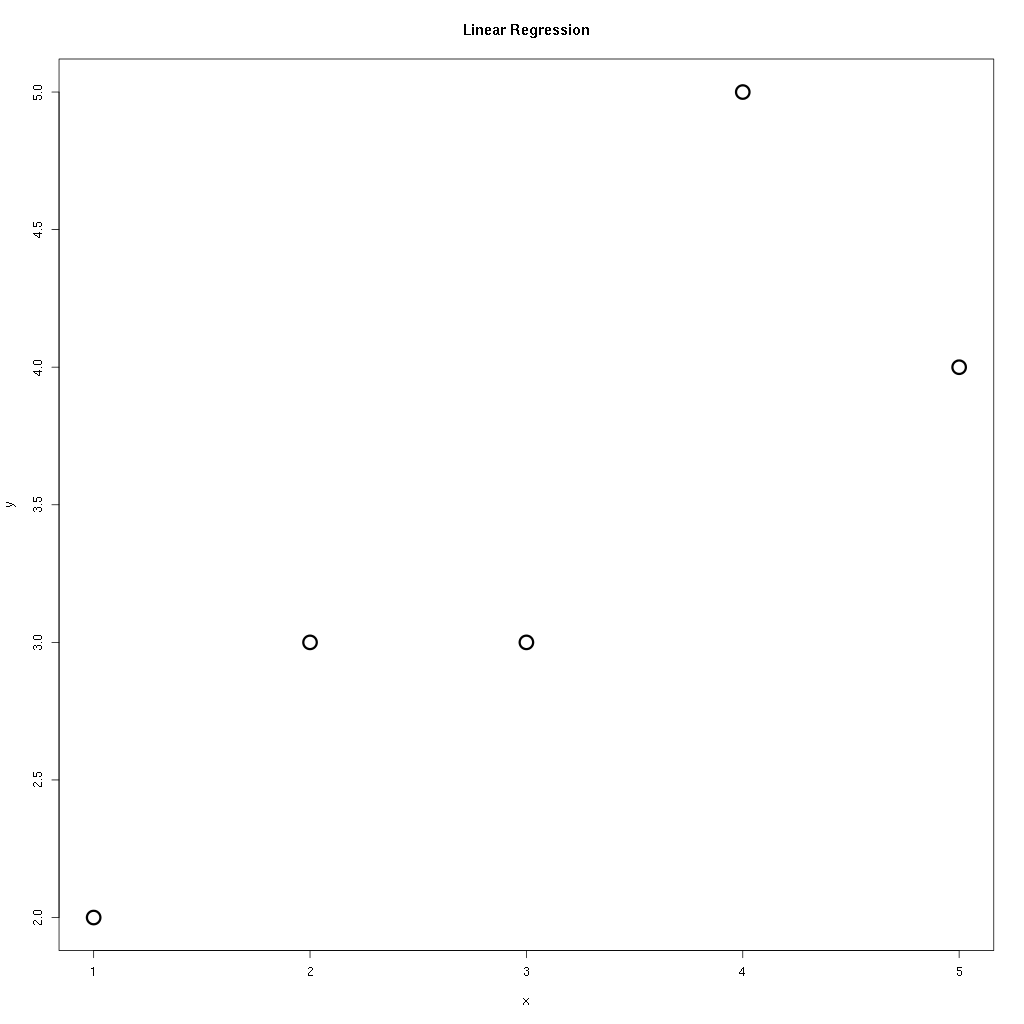
\includegraphics[width=4cm]{img/scatterLR-raw}}}
  \only<2>{\centerline{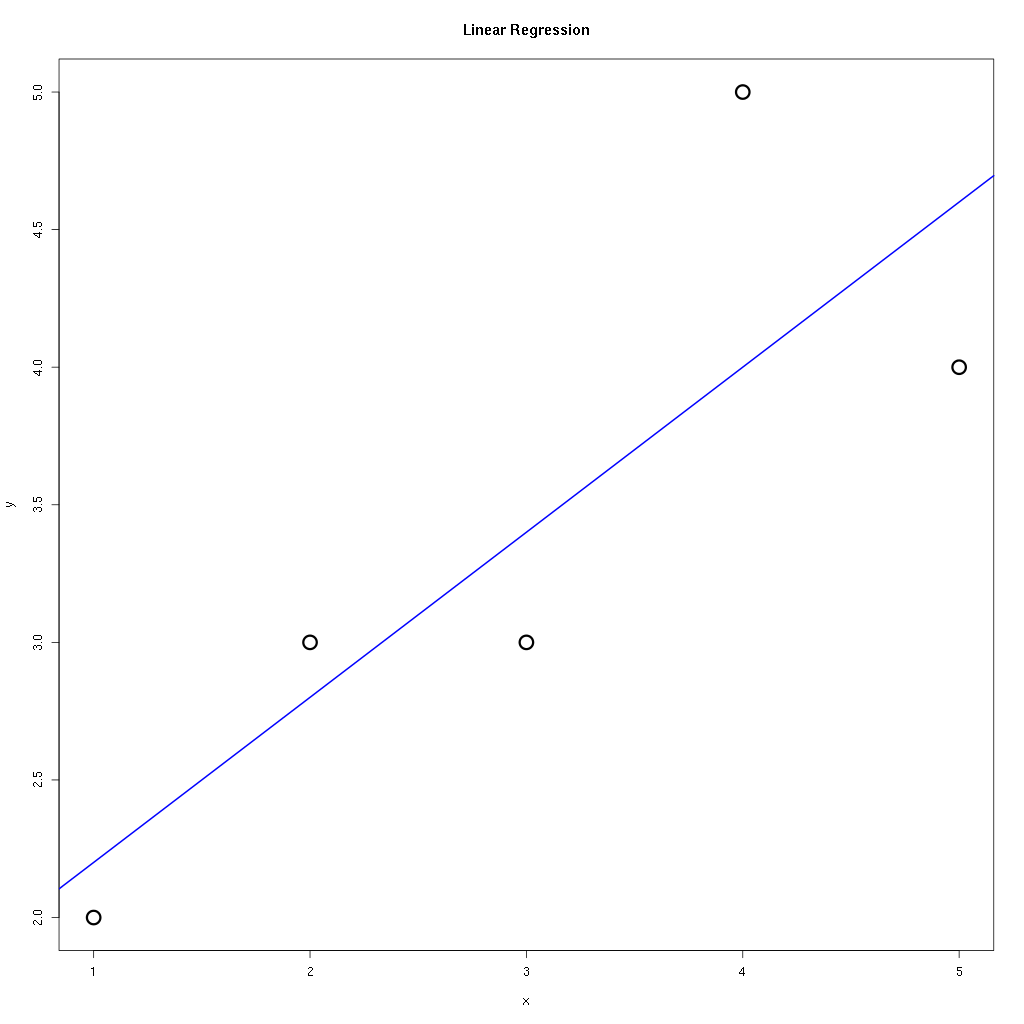
\includegraphics[width=4cm]{img/scatterLR-line}}}
  \only<3>{\centerline{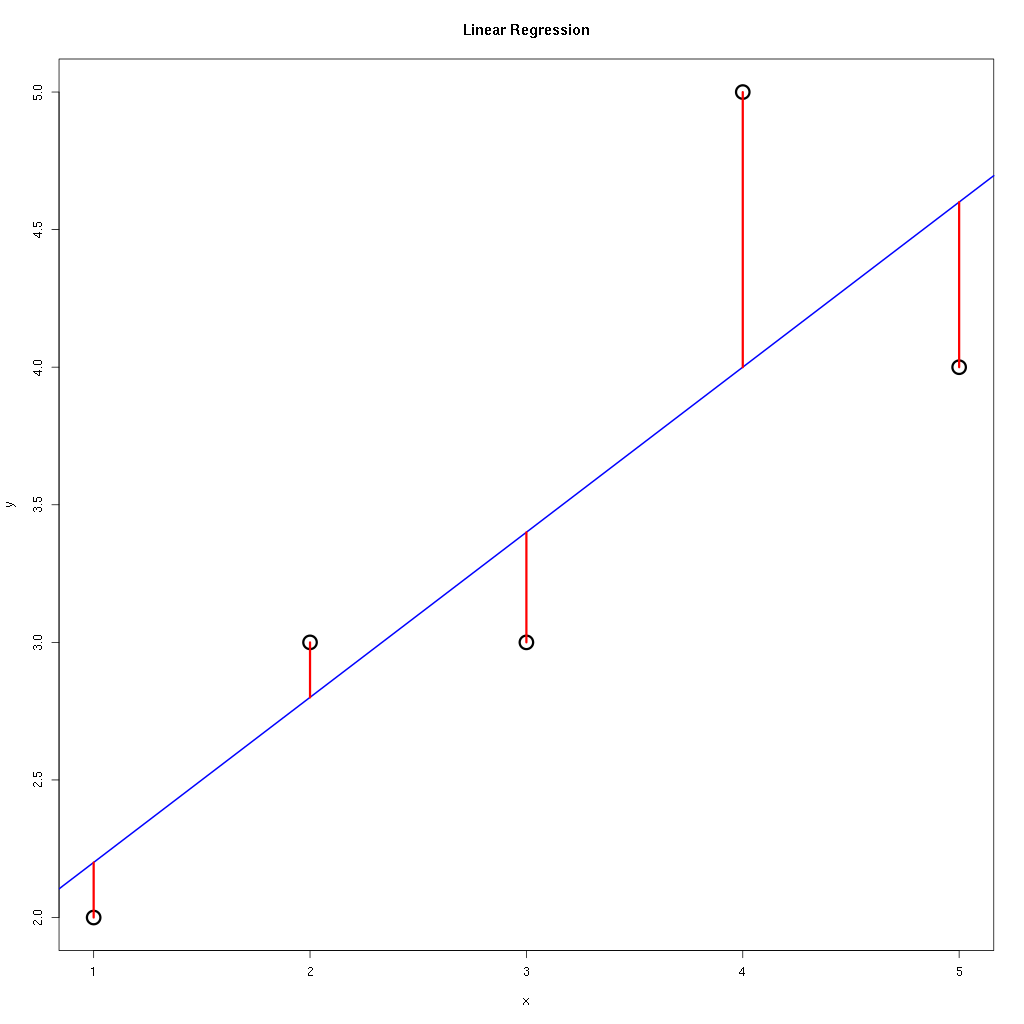
\includegraphics[width=4cm]{img/scatterLR-preResidual}}}
  \only<4->{%

    \centerline{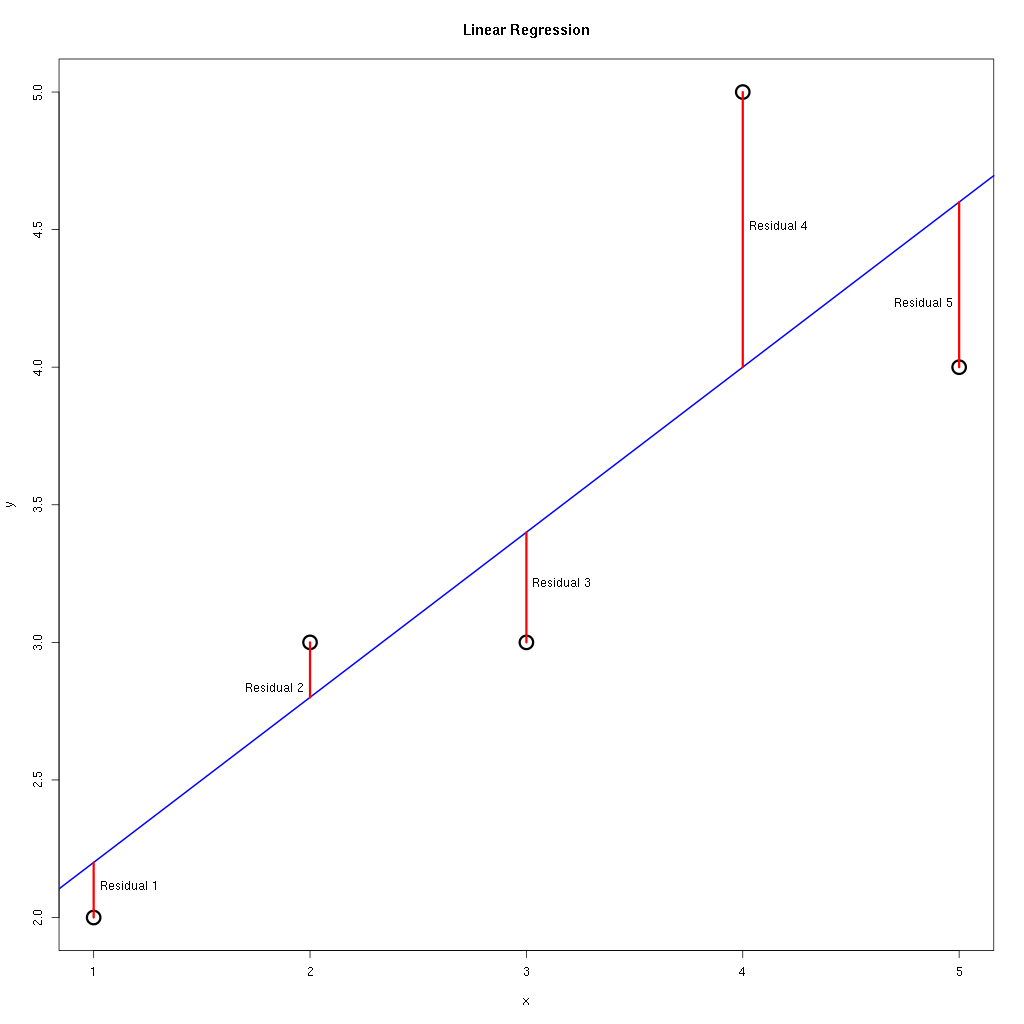
\includegraphics[width=4cm]{img/scatterLR-Residual}}
    
    \only<5->{%
      Goal: minimize
      \begin{eqnarray*}
        & & \lp\mathrm{residual~1}\rp^2 + \lp\mathrm{residual~2}\rp^2 + \\
        & & \lp\mathrm{residual~3}\rp^2 + \lp\mathrm{residual~4}\rp^2 + \lp\mathrm{residual~5}\rp^2 
      \end{eqnarray*}
    }

  }
  
\end{frame}

\begin{frame}
  \frametitle{Linear Regression}

    \begin{columns}
      \column{.65\textwidth}

      \centerline{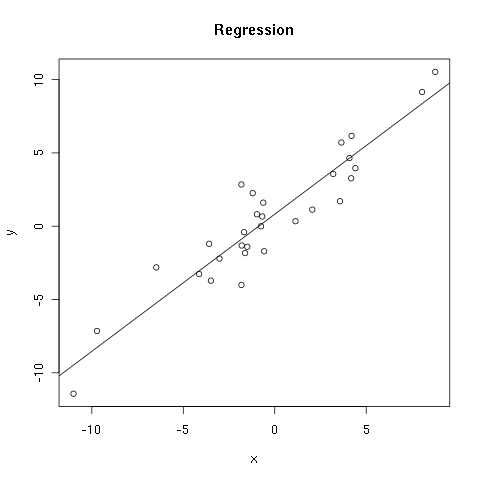
\includegraphics[width=6cm]{img/regressionGeneral}}

      \column{.35\textwidth}
      
      Our \textit{approximation} for the best linear fit is
      \begin{eqnarray*}
        y & = & \hat{m} x + \hat{b}.
      \end{eqnarray*}
      where
      \begin{eqnarray*}
        \hat{m} & = & \frac{s_{xy}}{s_{xx}}, \\
        \hat{b} & = & \bar{y} - \hat{m} \bar{x}.
      \end{eqnarray*}

    \end{columns}

\end{frame}


\begin{frame}{The Residual}

  \begin{definition}
    The \textit{\color{red} predicted value} for $y$ at $x_i$ is
    \begin{eqnarray*}
      \hat{y}_i & = & \hat{m} x_i + \hat{b}.
    \end{eqnarray*}

    The \textit{\color{red} residual} at $x_i$ is 
    \begin{eqnarray*}
      \mathrm{Residual} & = & y_i - \lp \hat{m} x_i + \hat{b} \rp, \\
      & = & y_i - \hat{y}_i.
    \end{eqnarray*}

  \end{definition}

  \only<2->
  {

    \begin{definition}
      The variance of the error is 
      \begin{eqnarray*}
        s^2_y & = & \frac{\lp y_1 - \hat{y}_1\rp^2 + \lp y_2 - \hat{y}_2\rp^2 + \cdots + \lp y_n - \hat{y}_n\rp^2 }{n-2}.
      \end{eqnarray*}
    \end{definition}

  }
  
\end{frame}

\begin{frame}{Example}

    \begin{columns}
      \column{.25\textwidth}

      \begin{tabular}{l|l}
        $X$ & $Y$ \\ \hline
        1 & 2 \\
        2 & 3  \\
        3 & 3 \\
        4 & 5  \\
        5 & 4
      \end{tabular}

      \column{.65\textwidth}

      \only<2>{%
        \centerline{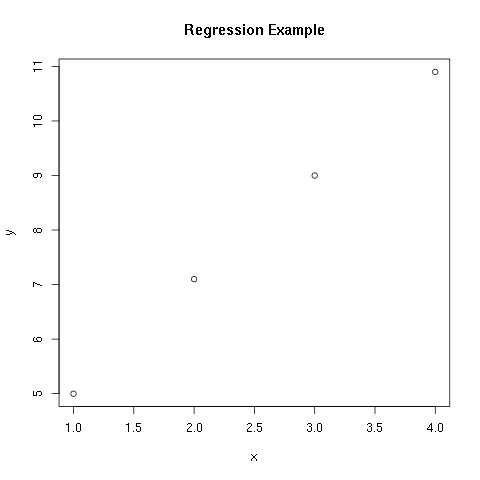
\includegraphics[width=4cm]{img/regressionExample}}
      }

      \only<3>{%
        \centerline{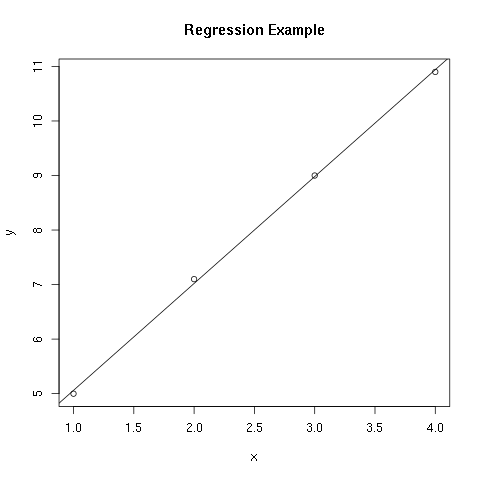
\includegraphics[width=4cm]{img/regressionExampleLine}}
      }


      \only<4->{%
        \begin{eqnarray*}
          \bar{x} & = & 3 \\
          \bar{y} & = & 3.4 \\
          s_{xx} & = & 10, \\
          s_{yy} & = & 5.2, \\
          s_{xy} & = & 6
        \end{eqnarray*}
      }

      \end{columns}

  \only<5->
  {

    \begin{eqnarray*}
      \hat{m} & = & \frac{s_{xy}}{s_{xx}}, \\
      & = & 0.6, \\
      \hat{b} & = & \bar{y} - \hat{m} \bar{x}, \\
      & = & 1.6
    \end{eqnarray*}

  }

  
\end{frame}



\begin{frame}{Example}

    \begin{columns}
      \column{.25\textwidth}

      \begin{tabular}{l|l}
        $X$ & $Y$ \\ \hline
        1 & 2 \\
        2 & 3  \\
        3 & 3 \\
        4 & 5  \\
        5 & 4
      \end{tabular}

      \column{.65\textwidth}

        \begin{eqnarray*}
          \bar{x} & = & 3 \\
          \bar{y} & = & 3.4 \\
          s_{xx} & = & 10, \\
          s_{yy} & = & 5.2, \\
          s_{xx} & = & 6, \\
          \hat{m} & = & 0.6, \\
          \hat{b} & = & 1.6
        \end{eqnarray*}

      \end{columns}

  \only<2->
  {

      \begin{tabular}{r|r<{\onslide<3->}|r<{\onslide<4->}|r<{\onslide}} % 
        $X$ & $Y$ & $\hat{Y}$ & Residual \\ \hline
        1 & 2 & 2.2 & -.2 \\
        2 & 3 & 2.8 &  .2 \\
        3 & 3 & 3.4 & -.4 \\
        4 & 5 & 4.0 & 1.0  \\
        5 & 4 & 4.6 & -.6
      \end{tabular}


  }

  
\end{frame}

\subsection{Inference for the Slope}

\begin{frame}{Example}

  \begin{tabular}{r|r|r|r}
    $X$ & $Y$ & $\hat{Y}$ & Residual \\ \hline
    1 & 2 & 2.2 & -.2 \\
    2 & 3 & 2.8 &  .2 \\
    3 & 3 & 3.4 & -.4 \\
    4 & 5 & 4.0 & 1.0  \\
    5 & 4 & 4.6 & -.6
  \end{tabular}

  \begin{eqnarray*}
    s^2_y & = & \frac{ (-.2)^2 + (.2)^2 + (-.4)^2 + (1.0)^2 + (-.6)^2}{5-2}, \\
    & = & \frac{1.6}{3}, \\
    s_y & = & \sqrt{\frac{1.6}{3}}, \\
    & \approx & .730
  \end{eqnarray*}
  
\end{frame}
  

\begin{frame}{What is the relationship?}


    \begin{columns}
      \column{.33\textwidth}

      \begin{eqnarray*}
        H_0: & & m=0, \\
        H_a: & & m<0,
      \end{eqnarray*}
      a negative relationship?

      \column{.33\textwidth}

      \begin{eqnarray*}
        H_0: & & m=0, \\
        H_a: & & m>0,
      \end{eqnarray*}
      a positive relationship?


      \column{.33\textwidth}

      \begin{eqnarray*}
        H_0: & & m=0, \\
        H_a: & & m\neq 0,
      \end{eqnarray*}
      any relationship?

      
    \end{columns}

  
\end{frame}





% LocalWords:  Clarkson pausesection hideallsubsections hideothersubsections
% LocalWords:  sectionstyle
